\documentclass[conference]{IEEEtran}

\usepackage{cite}
\usepackage{amsmath,amssymb,amsfonts}
\DeclareMathOperator{\Tr}{Tr}

\usepackage{subfigure}
\usepackage{booktabs}

\usepackage{bm}
\usepackage{graphicx}
\graphicspath{{../../../Figures/paper_19_05/}{../../../Images/paper_19_05/}}
\usepackage{textcomp}
\usepackage{xcolor}
\def\BibTeX{{\rm B\kern-.05em{\sc i\kern-.025em b}\kern-.08em
    T\kern-.1667em\lower.7ex\hbox{E}\kern-.125emX}}

\usepackage{balance}

\begin{document}

\title{Statistical Properties of Geodesic Distances between Samples and Elementary Backscatterers in PolSAR Imagery}

\author{\IEEEauthorblockN{Danilo Fernandes, 
Alejandro C.\ Frery,~\IEEEmembership{Senior Member,~IEEE}}
\IEEEauthorblockA{Laborat\'orio de Computa\c c\~ao Cient\'ifica e An\'alise Num\'erica\\
Universidade Federal de Alagoas\\
Macei\'o, Brazil\\
Email: dfc@laccan.ufal.br, acfrery@laccan.ufal.br
%acfrery@laccan.ufal.br
%\and  
%\IEEEauthorblockN{2\textsuperscript{nd} Danilo Fernandes}
%\IEEEauthorblockA{\textit{Laborat\'orio de Computa\c c\~ao Cient\'ifica e An\'alise Num\'erica} \\
%\textit{Universidade Federal de Alagoas}\\
%Macei\'o, Brazil \\
%dfc@laccan.ufal.br}
}}

\maketitle

\begin{abstract}
PolSAR data are usually represented by complex scattering or covariance matrices.
Another representation is by Kennaugh matrices, which are real and preserve the backscatter information.
This approach allows measuring distances and, consequently, the dissimilarity between PolSAR data and known backscatters.
In this report, we analyze the statistical properties of this dissimilarity measure between PolSAR data samples and elementary backscatters using a Geodesic Distance.
\end{abstract}

% Note that keywords are not normally used for peerreview papers.
\begin{IEEEkeywords}
PolSAR, Kennaugh matrix, Geodesic Distance.
\end{IEEEkeywords}

\section{Introduction}
\IEEEPARstart{I}{n} Polarimetric SAR, a radar target is characterized by a scattering matrix $\bm S$ that describes the dependence of its scattering properties on the polarization. 
It is defined as
\[\bm{S} = 
\begin{bmatrix}
S_{\text{HH}} & S_{\text{HV}}\\
S_{\text{VH}} & S_{\text{VV}}\\
\end{bmatrix}
,\]
where $\text{H}$ and $\text{V}$ denote, respectively, horizontal and vertical polarization.

This information can be projected and then visualized using the Pauli vector representation:
$\bm{k} = 2^{-1/2} 
\begin{bmatrix}
S_{\text{HH}} + S_{\text{VV}} &S_{\text{HH}} - S_{\text{VV}} &2S_{\text{HV}}
\end{bmatrix}^T
$, 
where $T$ denotes transposition. 
Another important matrix in PolSAR theory is the coherency $\bm{T}$ obtained by:
$$
\bm{T} = \frac{1}{L} \sum_{\ell=1}^{L}\textbf{k}_\ell \textbf{k}_\ell^{*T},
$$
where $*$ denotes the complex conjugate, and $L$ is the number of looks.

The Kennaugh matrix $\bm{K}$ can be obtained from the coherency matrix $\bm{T}$:
\[
\begin{bmatrix}
\frac{ T_{11} + T_{22} + T_{33} }{2} & \Re(T_{12}) & \Re(T_{13}) & \Im(T_{23})\\
\Re(T_{12}) & \frac{T_{11} + T_{22} - T_{33}}{2} & \Re(T_{23}) & \Im(T_{13})\\
\Re(T_{13}) & \Re(T_{23}) & \frac{ T_{11} - T_{22} + T_{33} }{2} & -\Im(T_{12})\\
\Im(T_{23}) & \Im(T_{13}) & -\Im(T_{12}) & \frac{ -T_{11} + T_{22} + T_{33} }{2}\\
\end{bmatrix}
.\]

The Geodesic Distance between two Kennaugh matrices $\bm K_1$ and $\bm K_2$ is~\cite{ClassificationPolSARGeodesic}: 
\begin{displaymath}
\text{GD}(\bm K_1, \bm K_2) = \frac{2}{\pi} \cos^{-1} \left(\frac{\Tr(\bm K_1^T \bm K_2)}{\sqrt{\Tr(\bm K_1^T \bm K_1)} \sqrt{\Tr(\bm K_2^T \bm K_2})} \right),
\end{displaymath}
where $\Tr$ denotes the trace.
It ranges between $[0,1]$.
This leads to defining a measure of similarity between PolSAR data: $f(\bm K_1, \bm K_2) = 1 - \text{GD}(\bm K_1, \bm K_2)$. 
This measure of dissimilarity has been used to 
classify images~\cite{ClassificationPolSARGeodesic},
in the proposal of a new generalized volume scattering model~\cite{AGeneralizedVolumeScatteringModelBasedVegetationIndexfromPolarimetricSARData2019},
and for the analysis of built-up areas~\cite{NovelTechniquesforBuiltupAreaExtractionfromPolarimetricSARImages2019}.
A measure of similarity, often more convenient for classification purposes~\cite{FreryCorreiaFreitas:ClassifMultifrequency:IEEE:2007}, is $1-\text{GD}$.

In this work, we are interested in the similarity between samples and elementary backscatterers:
trihedral, dihedral, random volume, narrow dihedral, cylinder, dipole, left helix, right helix, $+1/4$-wave and $-1/4$-wave, whose Kennaugh matrices are, respectively:
\begin{align*}
K_a &=
\begin{bmatrix}
1 & 0 & 0 & 0\\
0 & 1 & 0 & 0\\
0 & 0 & 1 & 0\\
0 & 0 & 0 & -1\\
\end{bmatrix},
K_b =
\begin{bmatrix}
1 & 0 & 0 & 0\\
0 & 1 & 0 & 0\\
0 & 0 & -1 & 0\\
0 & 0 & 0 & 1\\
\end{bmatrix},\\
K_{rv} &=
\begin{bmatrix}
1 & 0 & 0 & 0\\
0 & 1/2 & 0 & 0\\
0 & 0 & 1/2 & 0\\
0 & 0 & 0 & 0\\
\end{bmatrix},
K_{nd} =
\begin{bmatrix}
5/8 & 3/8 & 0 & 0\\
3/8 & 5/8 & 0 & 0\\
0 & 0 & -1/2 & 0\\
0 & 0 & 0 & 1/2
\end{bmatrix},\\
K_{c} &=
\begin{bmatrix}
5/8 & 3/8 & 0 & 0\\
3/8 & 5/8 & 0 & 0\\
0 & 0 & 1/2 & 0\\
0 & 0 & 0 & -1/2\\
\end{bmatrix},
K_d=
\begin{bmatrix}
1 & -1 & 0 & 0\\
-1 & 1 & 0 & 0\\
0 & 0 & 0 & 0\\
0 & 0 & 0 & 0\\
\end{bmatrix},\\
K_{lh} &=
\begin{bmatrix}
1 & 0 & 0 & -1\\
0 & 0 & 0 & 0\\
0 & 0 & 0 & 0\\
-1 & 0 & 0 & 1\\
\end{bmatrix},
K_{rh}=
\begin{bmatrix}
1 & 0 & 0 & 1\\
0 & 0 & 0 & 0\\
0 & 0 & 0 & 0\\
1 & 0 & 0 & 1\\
\end{bmatrix}
,\\
K_{+1/4} &=
\begin{bmatrix}
1 & 0 & 0 & 0\\
0 & 1 & 0 & 0\\
0 & 0 & 0 & 1\\
0 & 0 & 1 & 0\\
\end{bmatrix},
K_{-1/4}=
\begin{bmatrix}
1 & 0 & 0 & 0\\
0 & 1 & 0 & 0\\
0 & 0 & 0 & -1\\
0 & 0 & -1 & 0\\
\end{bmatrix}
.
\end{align*}

Table~\ref{tab:dist_matrix} presents the geodesic distances between these elementary backscatterers.
Fig.~\ref{fig:Network} shows a graphical representation of the relationships between them.
The width of the edges in this complete graph is proportional to the distance between each pair, as presented in Table~\ref{tab:dist_matrix}.

\begin{table}[hbt]
\centering
\caption{The geodesic distance between elementary backscatterers}\label{tab:dist_matrix}
\begin{tabular}{lrrrrr}
\toprule
& $K_{a}$ & $K_{b}$ & $K_{rv}$ & $K_{nd}$ & $K_{c}$\\
\cmidrule(lr){2-6}
$K_{a}$ & 0.000 & 1.000 & 0.391 & 0.936 & 0.287\\
$K_{b}$ & 1.000 & 0.000 & 0.732 & 0.287 & 0.936\\
$K_{rv}$ & 0.391 & 0.732 & 0.000 & 0.703 & 0.434\\
$K_{nd}$ & 0.936 & 0.287 & 0.703 & 0.000 & 0.765\\
$K_{c}$ & 0.287 & 0.936 & 0.434 & 0.765 & 0.000\\
$K_{d}$ & 0.666 & 0.666 & 0.580 & 0.871 & 0.871\\
$K_{lh}$ & 1.000 & 0.666 & 0.732 & 0.702 & 0.968\\
$K_{rh}$ & 1.000 & 0.666 & 0.732 & 0.702 & 0.968\\
$K_{+1/4}$ & 0.666 & 0.666 & 0.580 & 0.666 & 0.666\\
$K_{-1/4}$ & 0.666 & 0.666 & 0.580 & 0.666 & 0.666\\
\midrule
& $K_{d}$ & $K_{lh}$ & $K_{rh}$ & $K_{+1/4}$ & $K_{-1/4}$\\
\cmidrule(lr){2-6}
$K_{a}$ & 0.666 & 1.000 & 1.000 & 0.666 & 0.666\\
$K_{b}$ & 0.666 & 0.666 & 0.666 & 0.666 & 0.666\\
$K_{rv}$ & 0.580 & 0.732 & 0.732 & 0.580 & 0.580\\
$K_{nd}$ & 0.871 & 0.702 & 0.702 & 0.666 & 0.666\\
$K_{c}$ & 0.871 & 0.968 & 0.968 & 0.666 & 0.666\\
$K_{d}$ & 0.000 & 0.839 & 0.839 & 0.666 & 0.666\\
$K_{lh}$ & 0.839 & 0.000 & 1.000 & 0.839 & 0.839\\
$K_{rh}$ & 0.839 & 1.000 & 0.000 & 0.839 & 0.839\\
$K_{+1/4}$ & 0.666 & 0.839 & 0.839 & 0.000 & 1.000\\
$K_{-1/4}$ & 0.666 & 0.839 & 0.839 & 1.000 & 0.000\\
\bottomrule
\end{tabular} 
\end{table}

\begin{figure}[hbt]
\centering
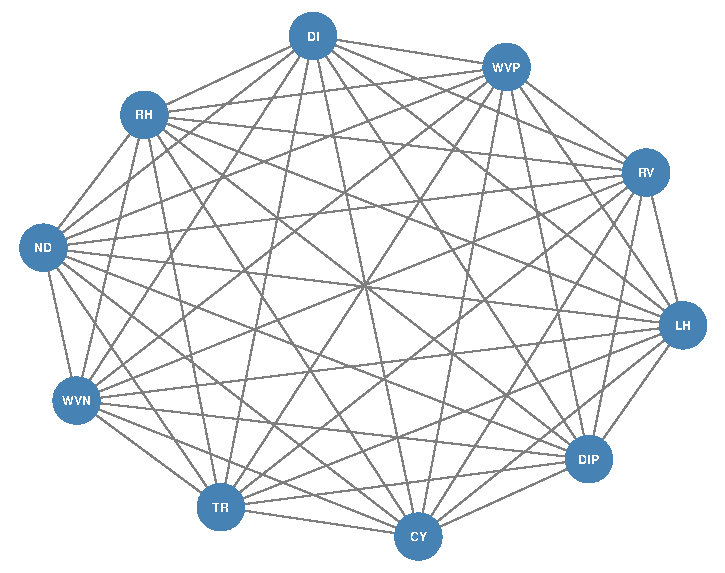
\includegraphics[width=.95\linewidth]{network}
\caption{Representation of the relationships among elementary backscatterers.}\label{fig:Network}
\end{figure}

The forthcoming section presents an empirical analysis of the similarities between the aforementioned elementary backscatters and PolSAR data from samples of vegetation and bare soil. 
The data is from UAVSAR image over Sierra del Lacandon National Park, Guatemala.
%%% ACF Se possível, forneça mais informações: data, banda, resolução espacial, número de looks etc.

\section{Analysis of Distances}

We selected samples of size $50\times 50$ pixels over forest and bare soil regions, and computed the similarities of the observation to each elementary backscatterer.
We also fitted a Beta distribution, with density given by
$$
\frac{\Gamma(\alpha+\beta)}{\Gamma(\alpha)\Gamma(\beta)}x^{\alpha-1}(1-x)^{\beta-1},
$$
with $x \in [ 0,1]$, $\alpha,\beta>0$.
Some of the similarities did not span the $[0,1]$ interval;
these cases were linearly mapped into this interval, and then fitted by the Beta law.

The mean is given by
\begin{equation}
  \mu = \frac{\alpha}{\alpha + \beta}.
  \label{eq:MeanBeta}
\end{equation}
We estimated $\alpha$ and $\beta>0$ by maximum likelihood and, thus, obtained models for these similarities.

We selected visually homogeneous regions of size $50\times50$ pixels from forested and bare soil areas.
They are shown, in Pauli decomposition, in Figs.~\ref{fig:forest} and \ref{fig:bare_soil}, respectively.



The histograms of the similarity of these data to each elementary backscatterer are shown in Figs.~\ref{fig:wvn} to \ref{fig:tr}.


\begin{figure}[hbt]
    \vspace{.1\linewidth}
    \centering
    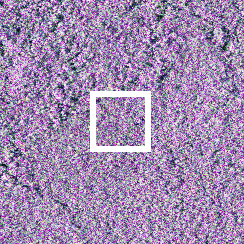
\includegraphics[width = .7\linewidth]{forest}
    \caption{Visualization of PolSAR data from the forest region through Pauli decomposition.}
    \label{fig:forest}
\end{figure}

\begin{figure}[hbt]
    \vspace{.1\linewidth}
    \centering
    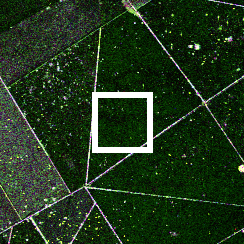
\includegraphics[width = .7\linewidth]{bare_soil.png}
    \caption{Visualization of PolSAR data from the bare soil region through Pauli decomposition.}
    \label{fig:bare_soil}
\end{figure}

%Code generator of these histograms is in Code folder in this repository
\begin{figure*}[hbt]
\centering
\subfigure[Similarity w.r.t. $-1/4$-wave elementary backscatterer\label{fig:wvn}]{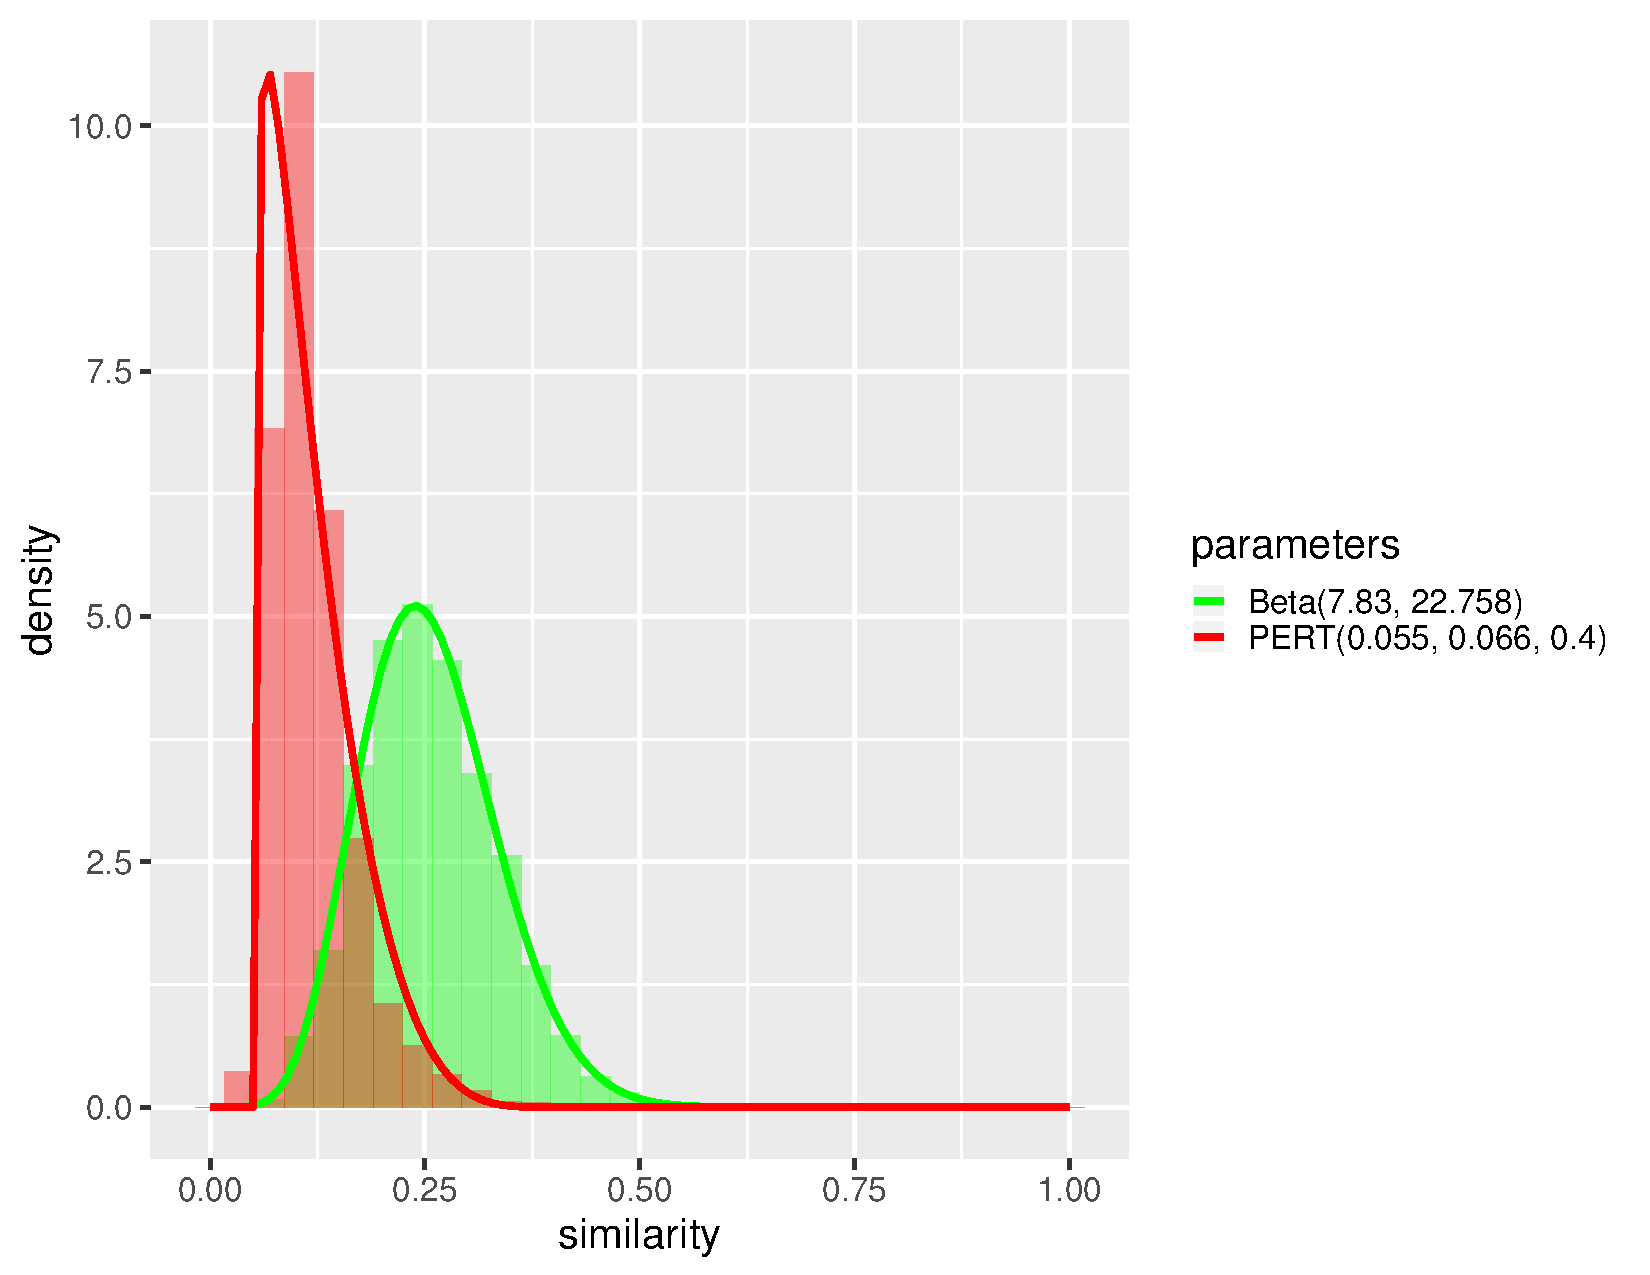
\includegraphics[width = .19\linewidth]{wvn}}
%
\subfigure[Similarity w.r.t. $+1/4$-wave elementary backscatterer\label{fig:wvp}]{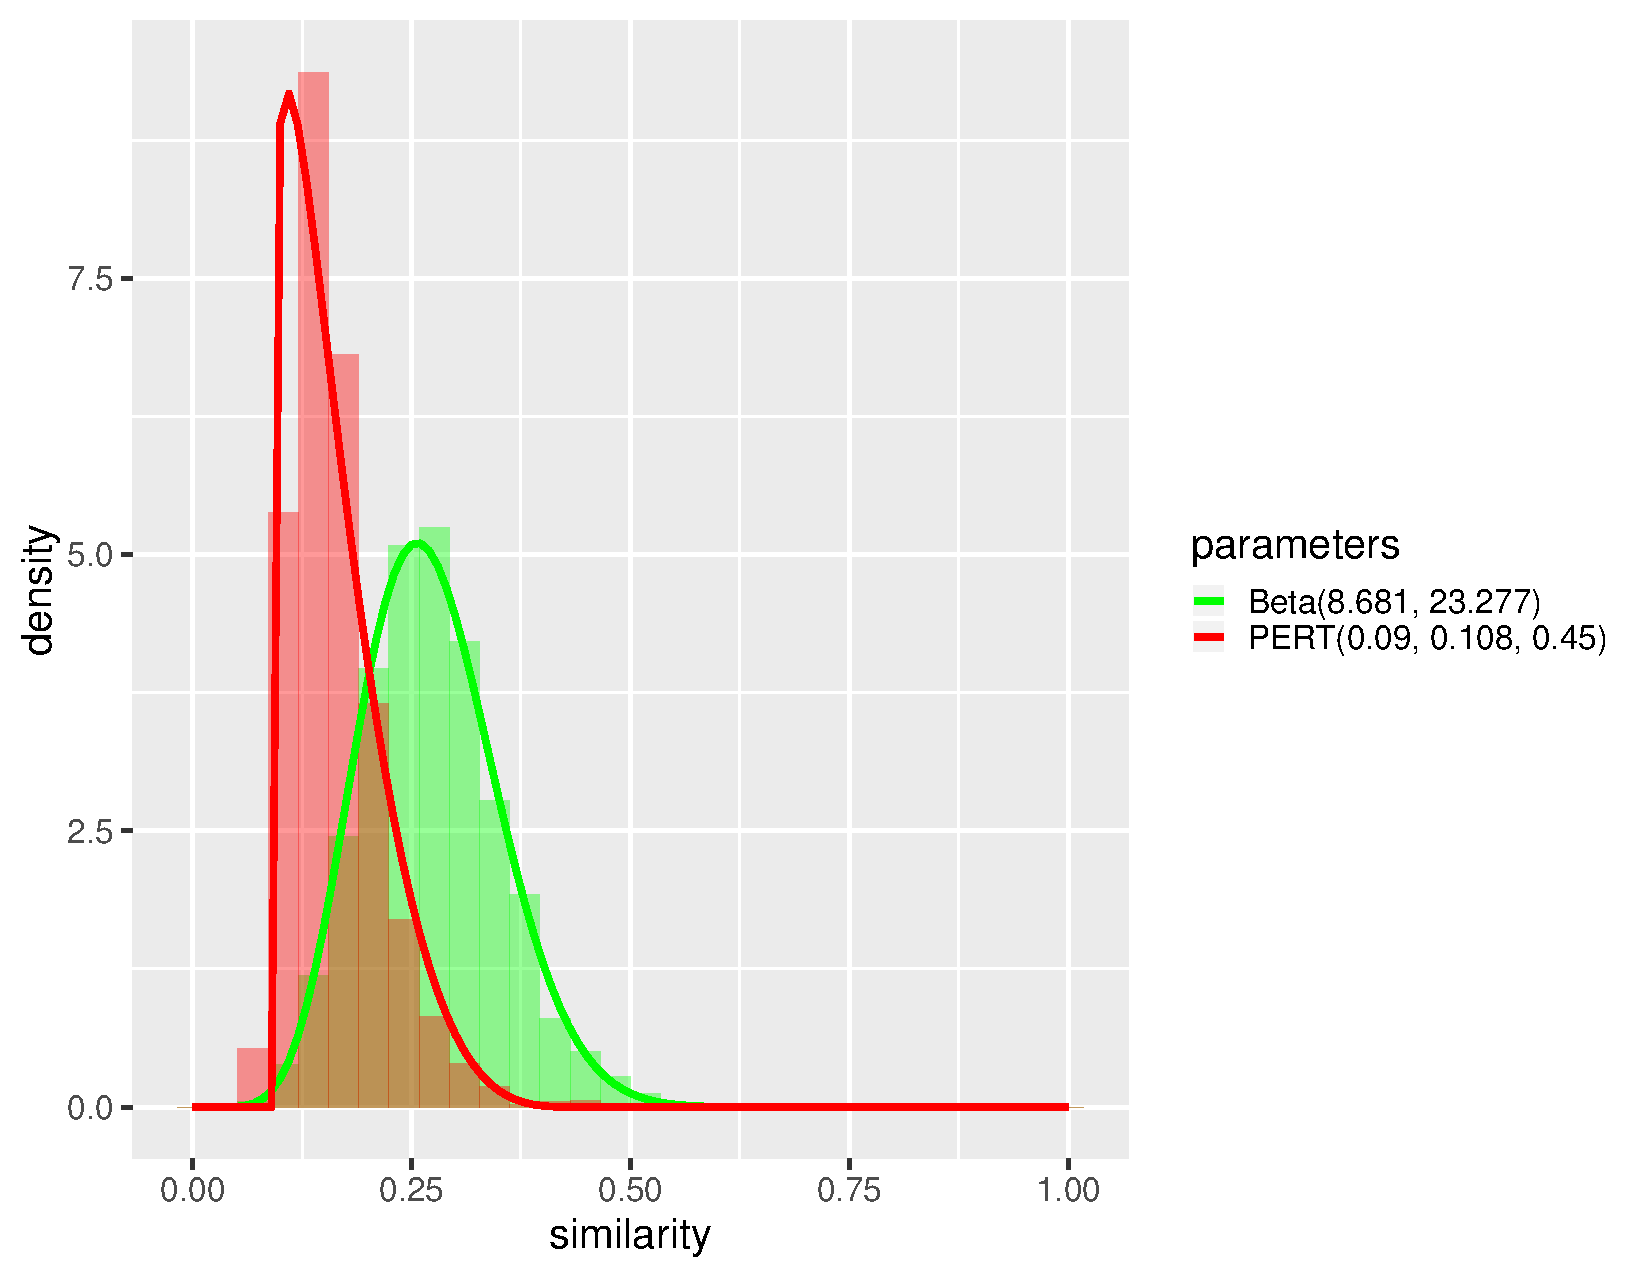
\includegraphics[width = .19\linewidth]{wvp}}
%
\subfigure[Similarity w.r.t. $+1/4$-wave elementary backscatterer\label{fig:cy}]{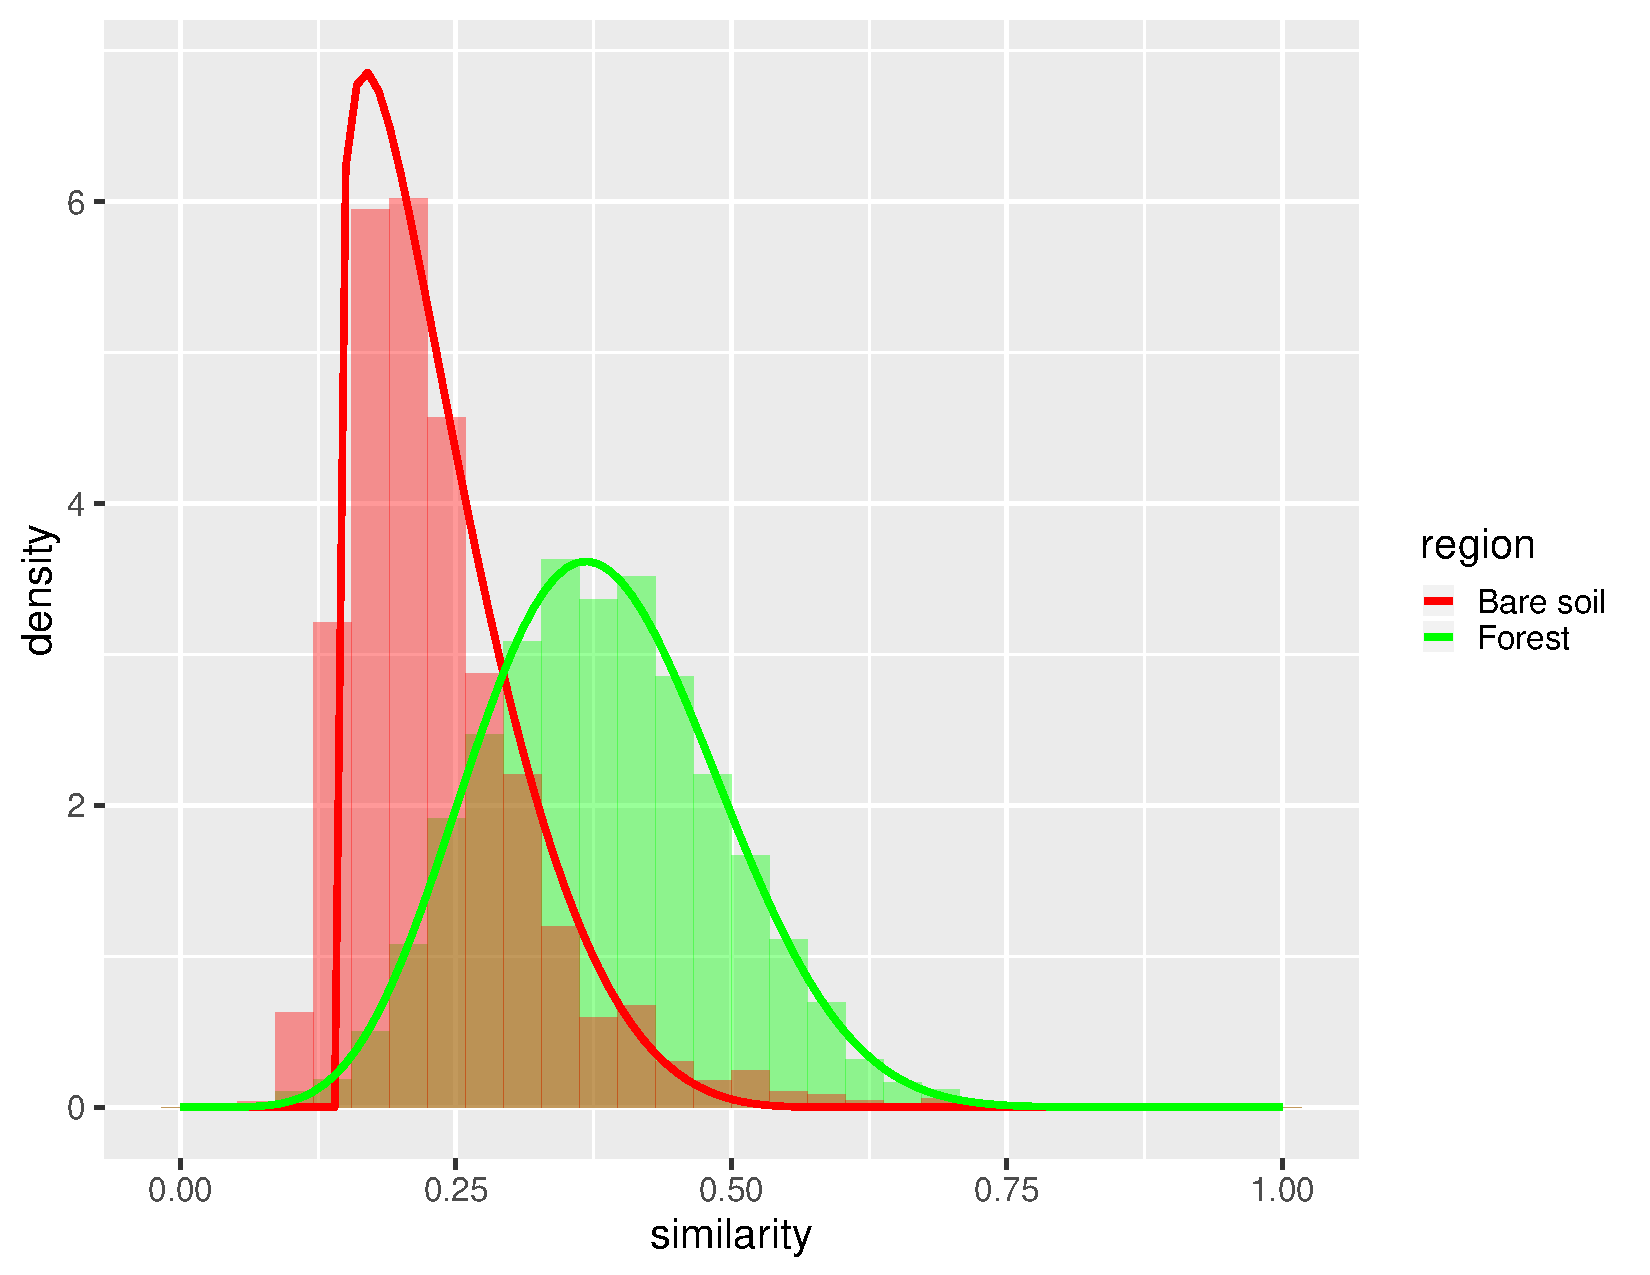
\includegraphics[width = .19\linewidth]{cy}}
%
\subfigure[Similarity w.r.t. dihedral elementary backscatterer\label{fig:di}]{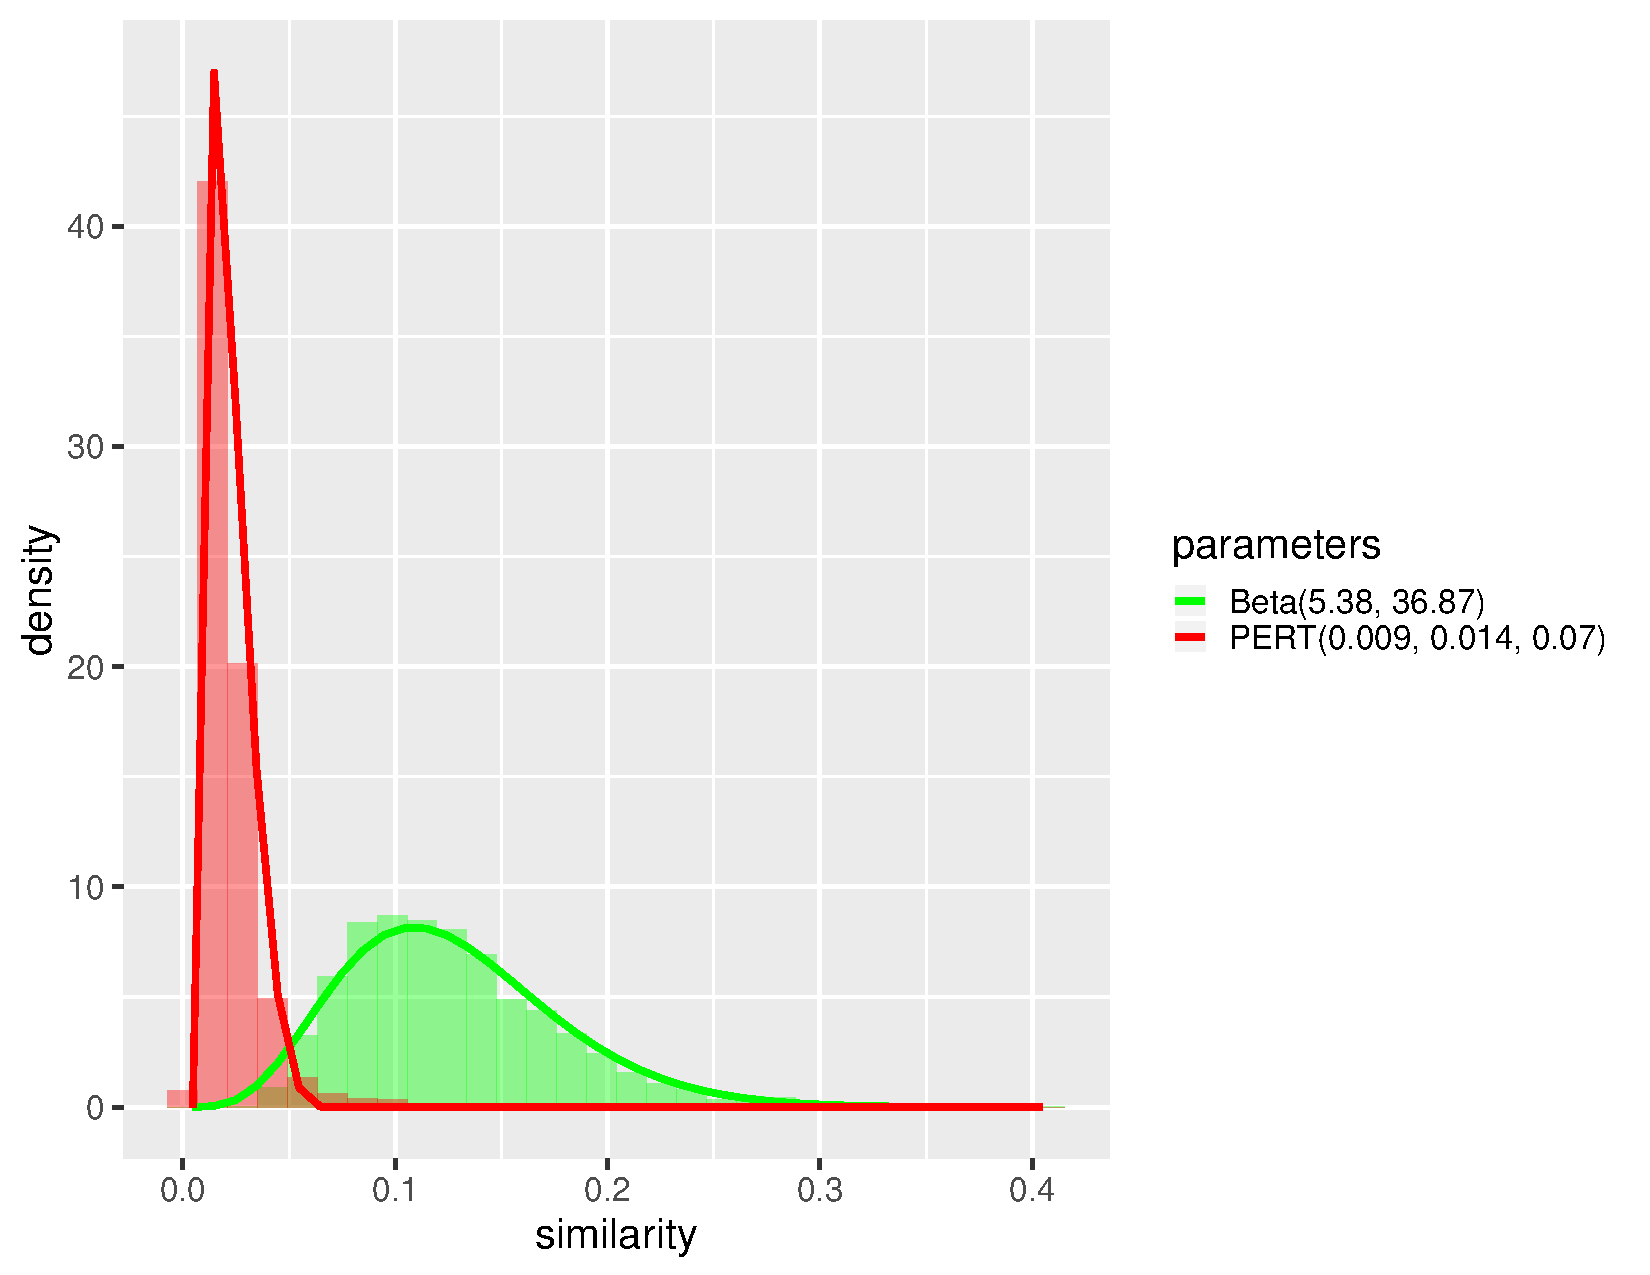
\includegraphics[width = .19\linewidth]{di}}
%
\subfigure[Similarity w.r.t. dipole elementary backscatterer\label{fig:dip}]{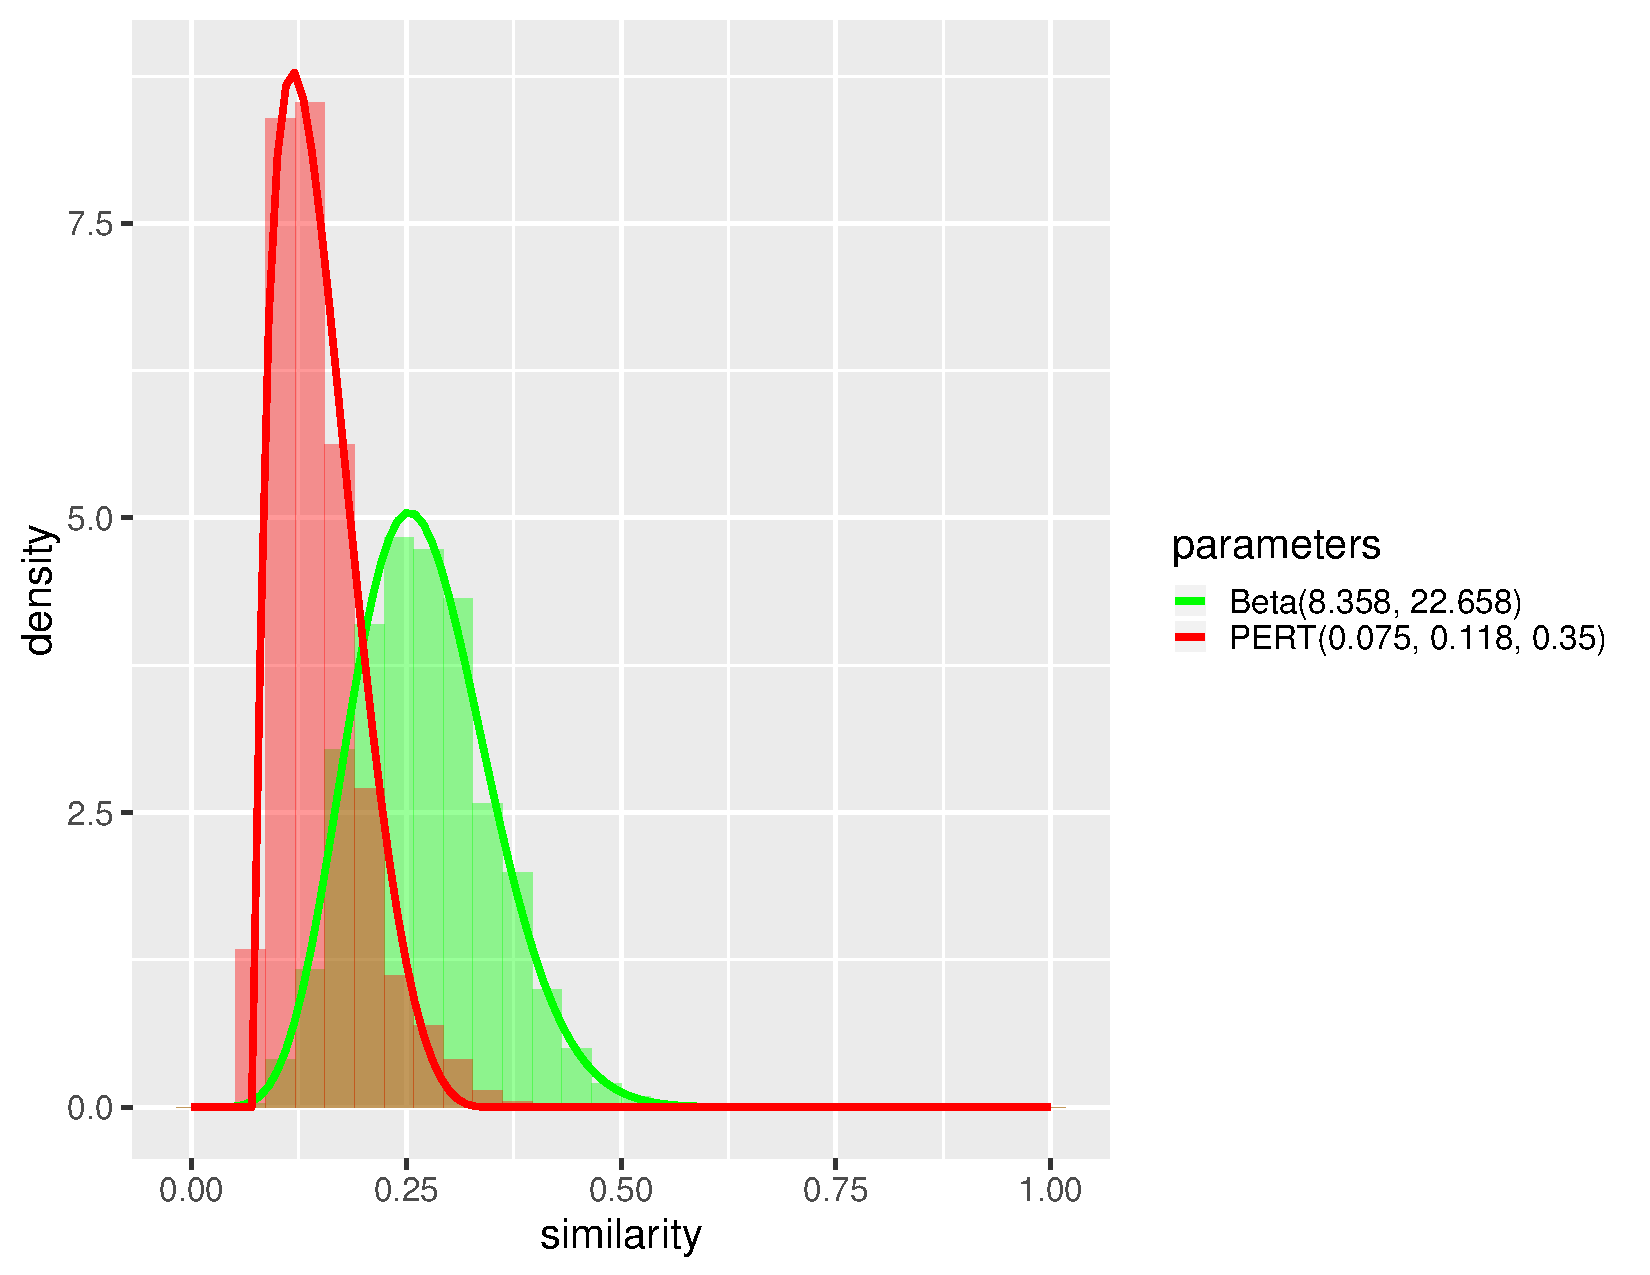
\includegraphics[width = .19\linewidth]{dip}}
%
\subfigure[Similarity w.r.t. narrow dihedral backscatterer\label{fig:nd}]{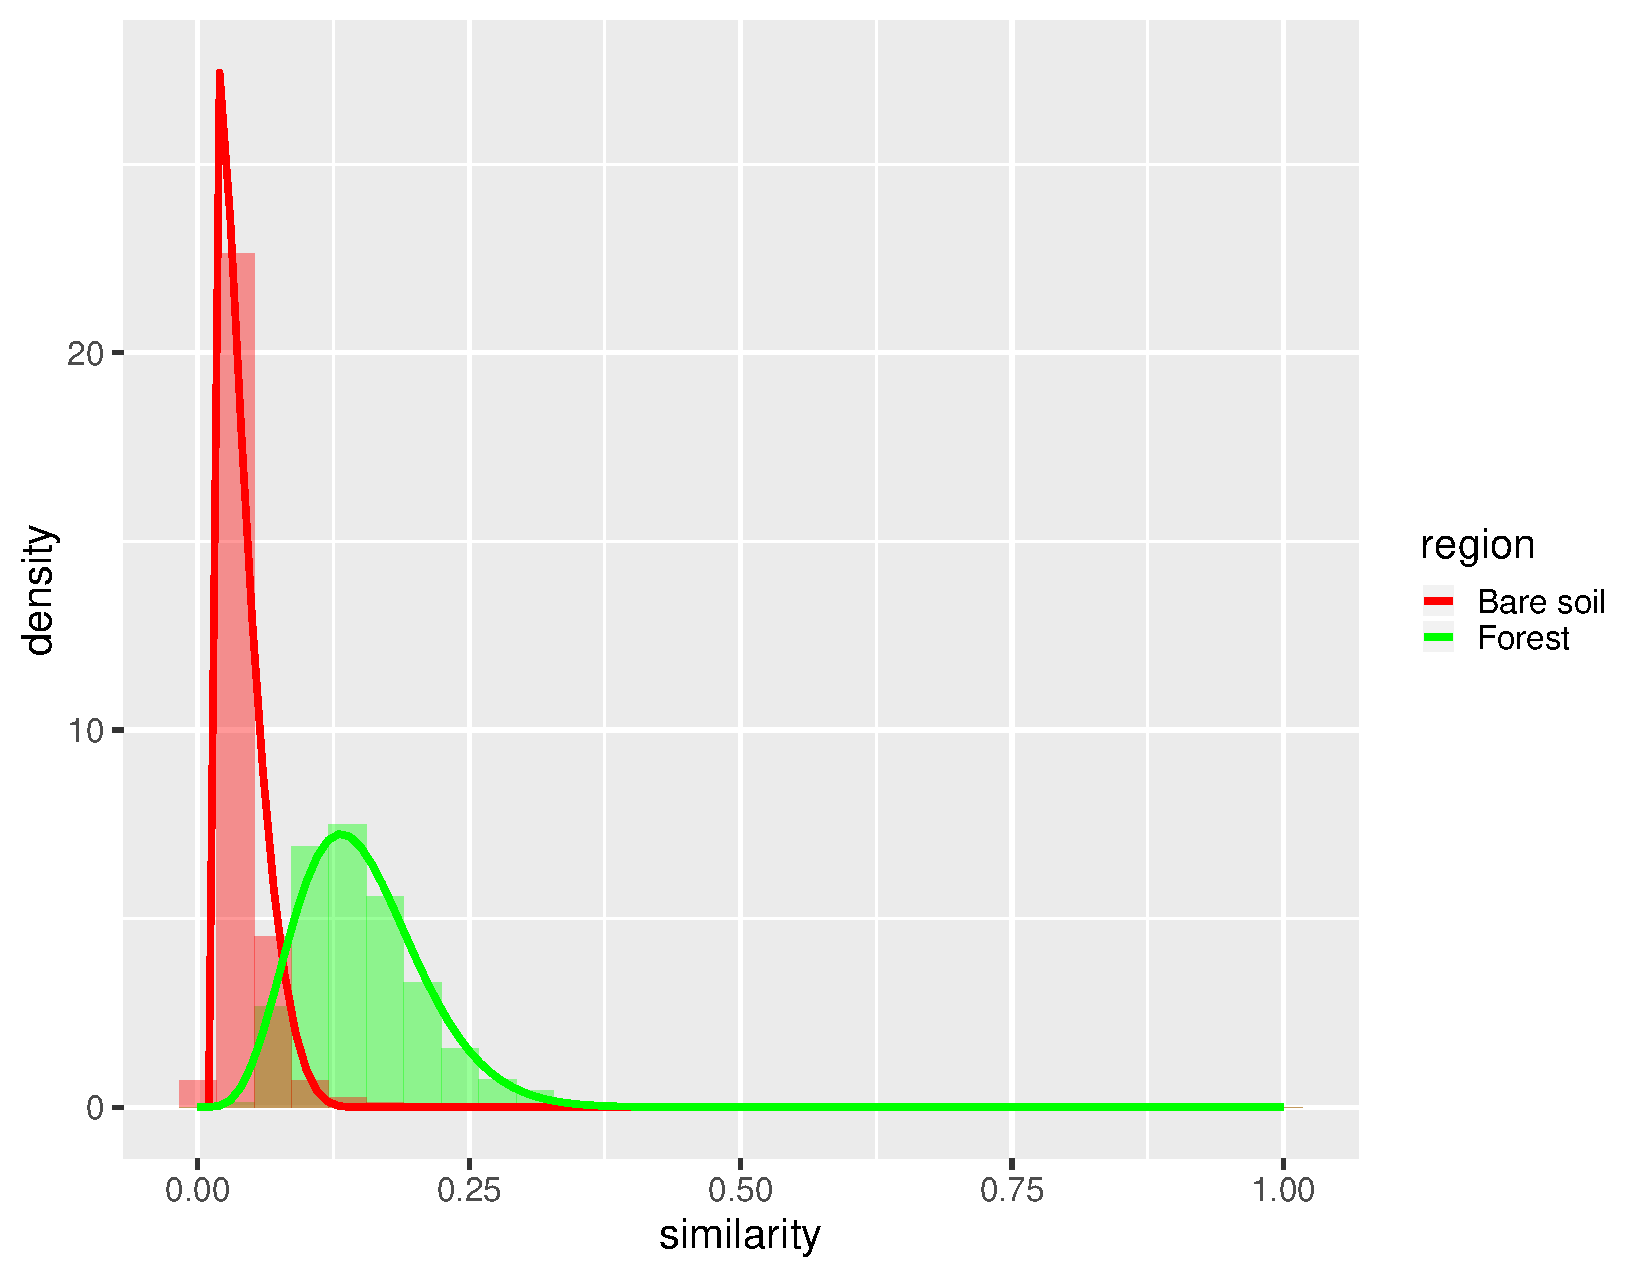
\includegraphics[width = .19\linewidth]{nd}}
%
\subfigure[Similarity w.r.t. left helix backscatterer\label{fig:lh}]{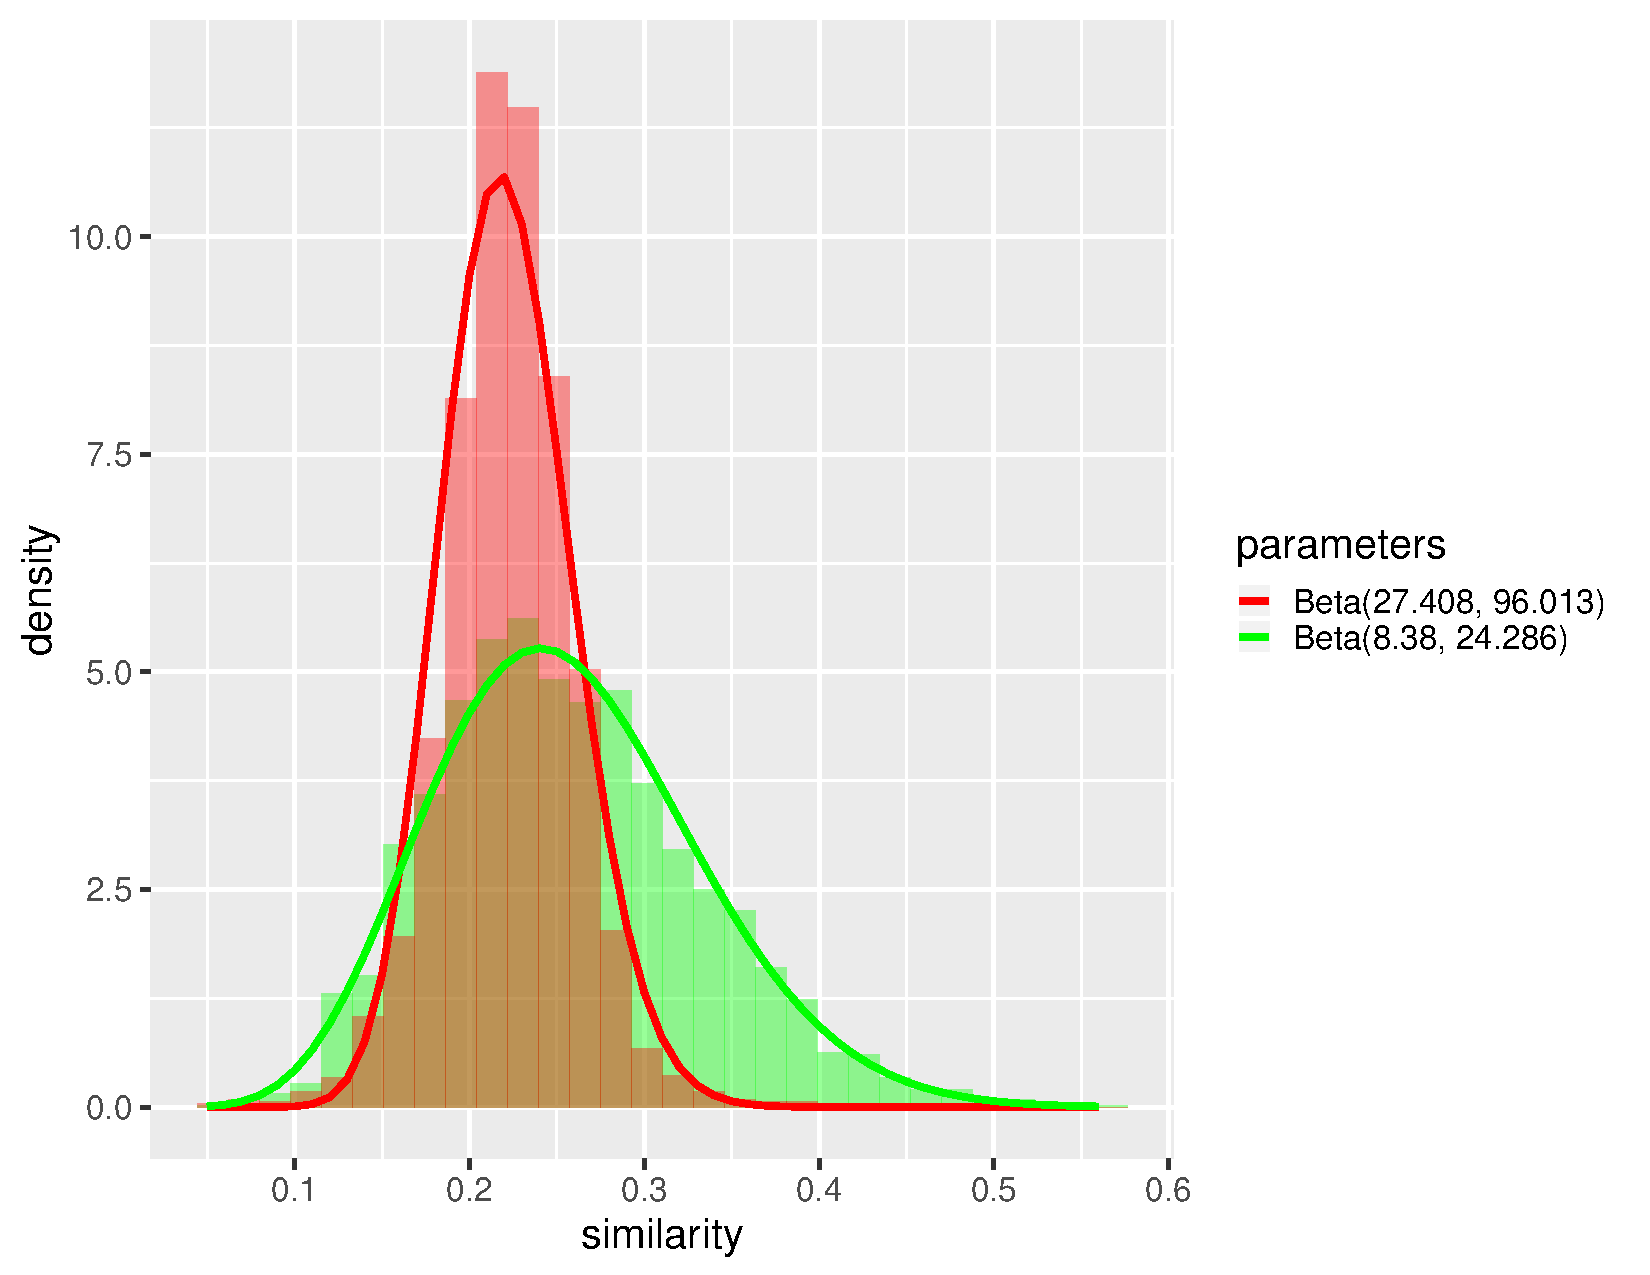
\includegraphics[width = .19\linewidth]{lh}}
%
\subfigure[Similarity w.r.t. right helix backscatterer\label{fig:rh}]{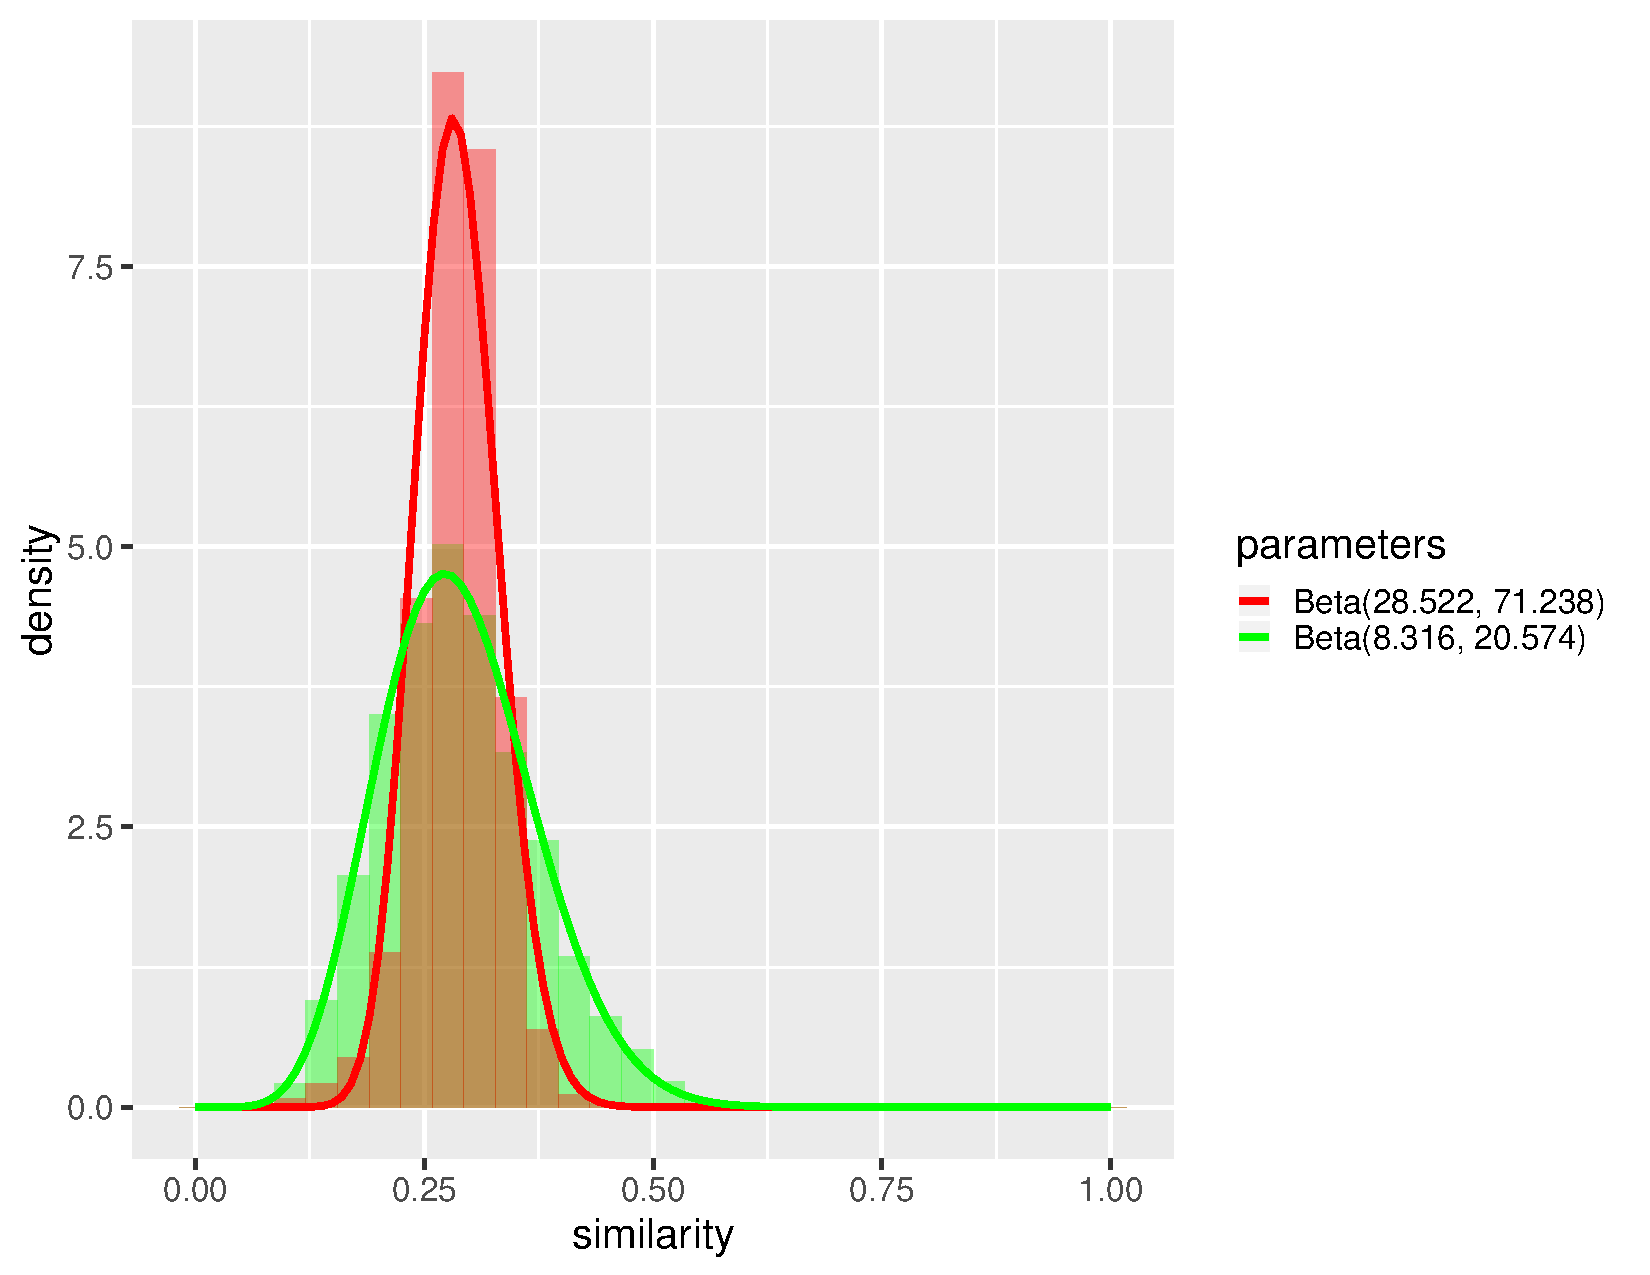
\includegraphics[width = .19\linewidth]{rh}}
%
\subfigure[Similarity w.r.t. random volume backscatterer\label{fig:rv}]{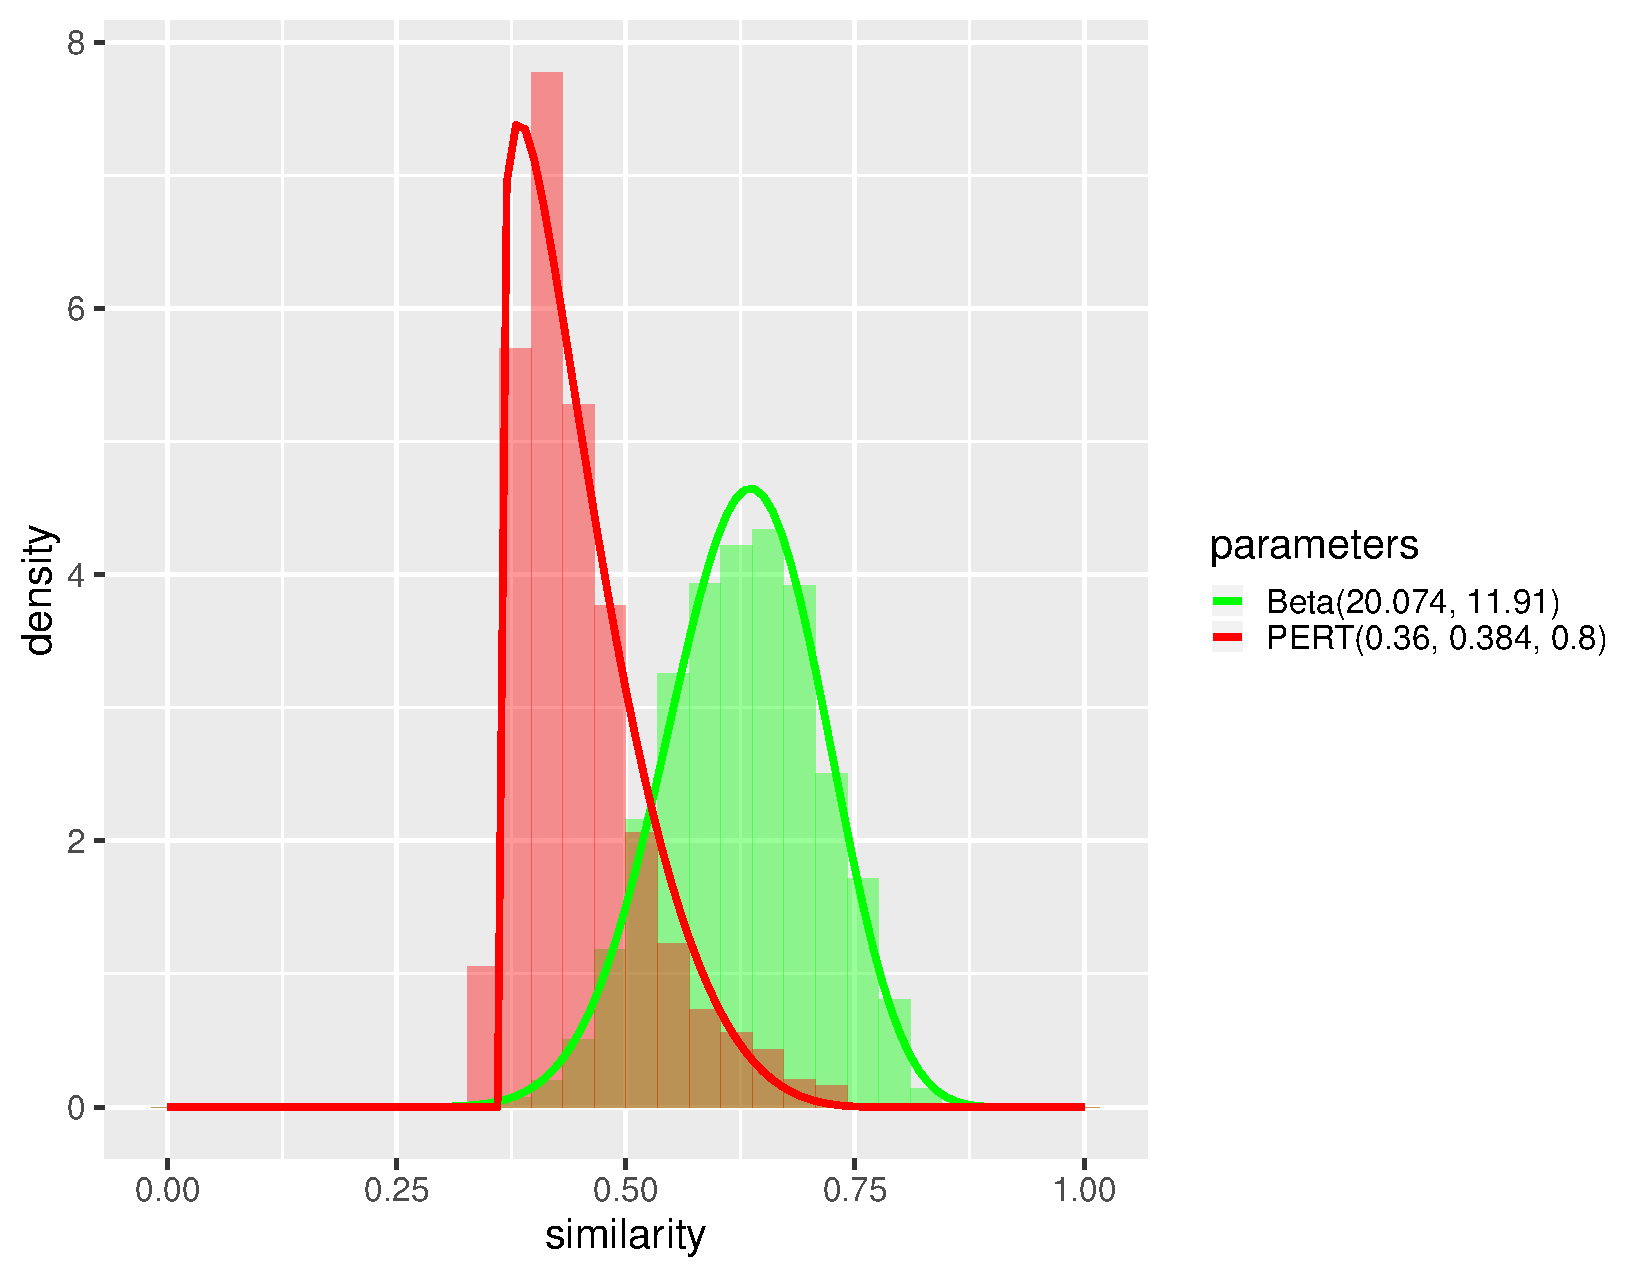
\includegraphics[width = .19\linewidth]{rv}}
%
\subfigure[Similarity w.r.t. trihedral backscatterer\label{fig:tr}]{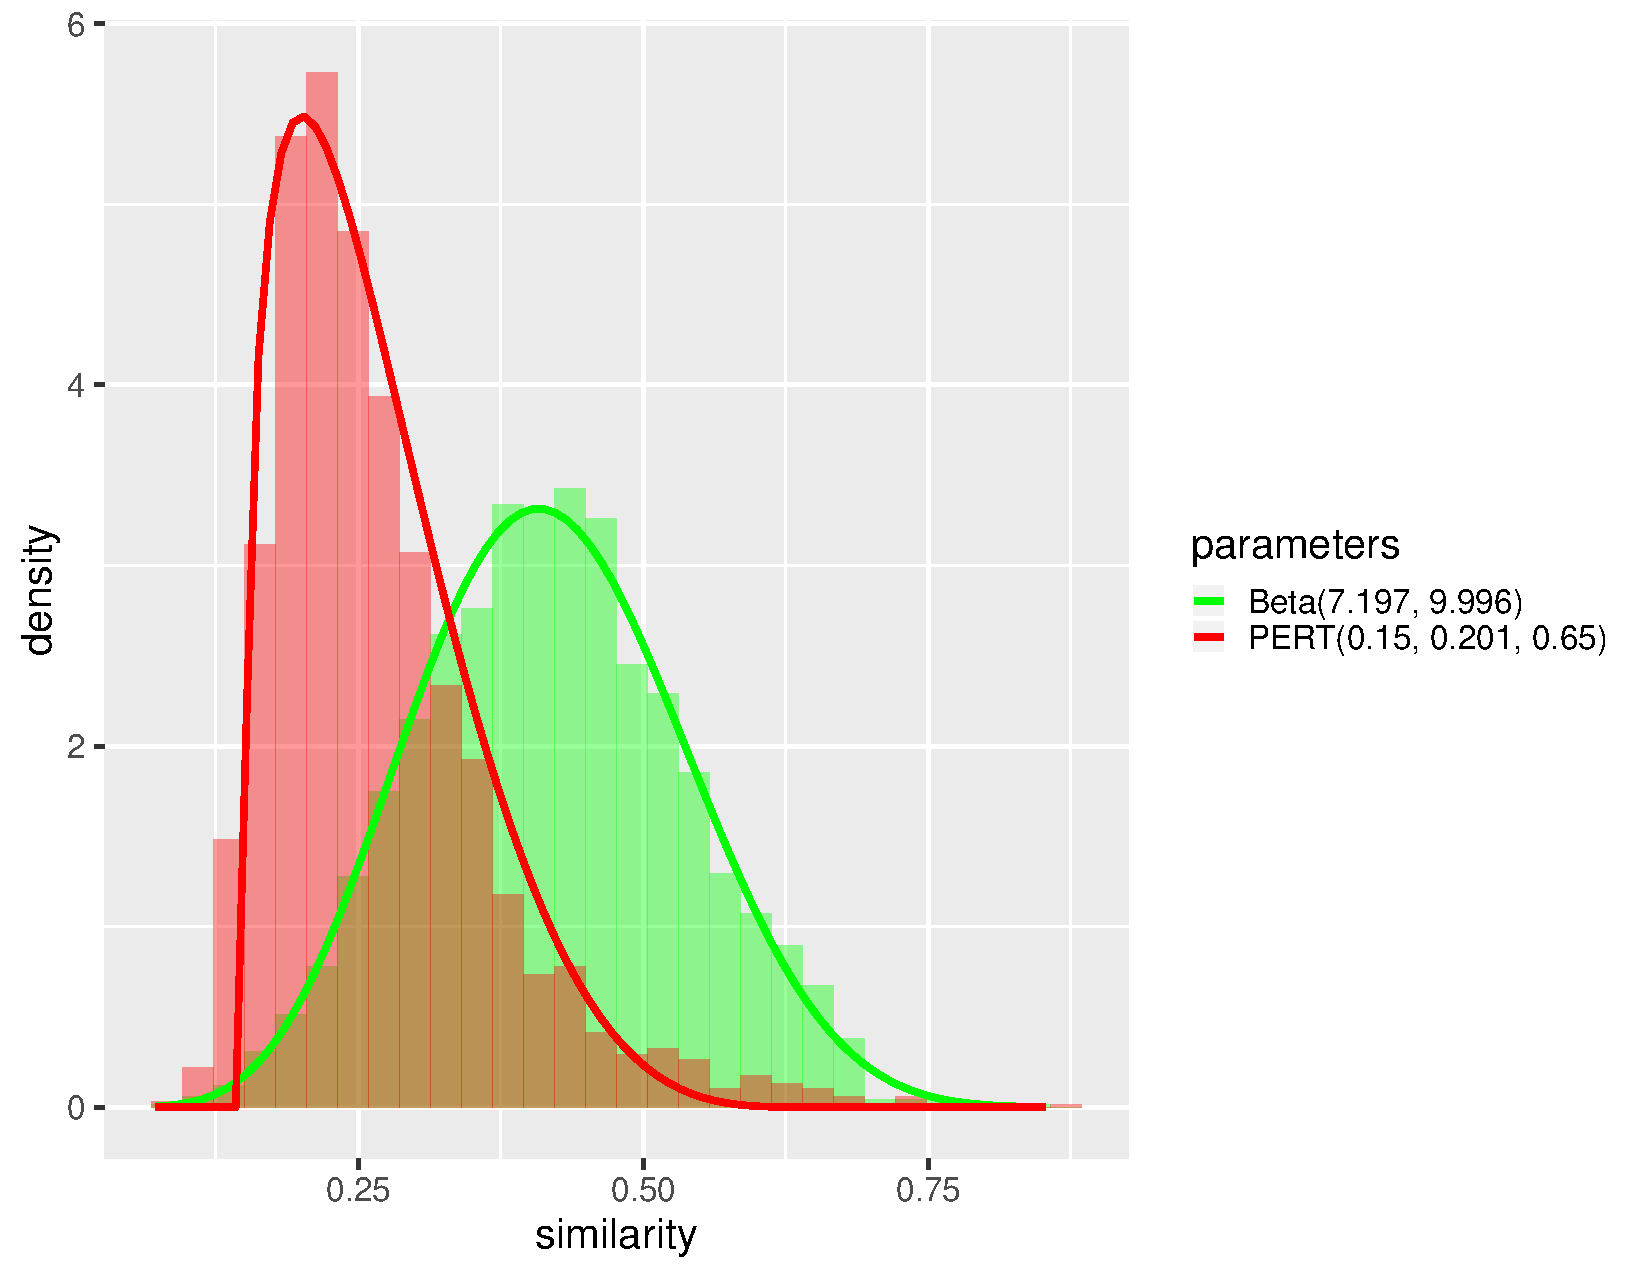
\includegraphics[width = .19\linewidth]{tr}}
\caption{Histograms of similarities between forest and bare soil samples with respect to ten elementary backscatterers; Forest in green, Bare Soil in red, overlap in brown.}\label{Fig:Histograms}
\end{figure*}

The differences are clear, denoting the expressiveness of this measure of similarity.

Table~\ref{tab:estimated_params} shows the estimated parameters of the Beta distribution when used as model for all similarities.
The table also presents the minima and maxima of each sample, and the estimate of the mean value computed with~\eqref{eq:MeanBeta}.

The elementary backscatterers which are closest to the samples are highlighted in red.
It is noteworthy that both Forest and Bare Soil are closest to the Random Volume model.

Through those, the probability density functions of the figures \ref{fig:wvn} to \ref{fig:tr} were adjusted to the histograms of the similarities. In addition, this table contains the estimate of the hope that results from the estimation of these parameters.

\balance
\begin{table}[hbt]
\centering
\caption{Estimates of the Beta distribution, minima, maxima, and estimated mean}\label{tab:estimated_params}     
\begin{tabular}{lrrrrr}
\toprule
& $\min$ & $\max$ & $\widehat\alpha$ & $\widehat\beta$ & $\widehat\mu$\\ \midrule
& \multicolumn{5}{c}{$-1/4$-wave}\\
\cmidrule(lr){2-6}
\textbf{Forest} & 0.000 & 1.000 & 7.830 & 22.758 & 0.255\\
\textbf{Bare soil} & 0.055 & 0.400 & 1.127 & 4.872 & 0.119\\
\midrule
%
& \multicolumn{5}{c}{$+1/4$-wave}\\
\cmidrule(lr){2-6}
\textbf{Forest} & 0.000 & 1.000 & 8.681 & 23.277 & 0.271\\
\textbf{Bare soil} & 0.090 & 0.450 & 1.200 & 4.800 & 0.162\\
\midrule
%
& \multicolumn{5}{c}{Cylinder}\\
\cmidrule(lr){2-6}
\textbf{Forest} & 0.000 & 1.000 & 7.500 & 12.165 & 0.381\\
\textbf{Bare soil} & 0.140 & 0.600 & 1.243 & 4.756 & 0.235\\
\midrule
%
& \multicolumn{5}{c}{Dihedral}\\
\cmidrule(lr){2-6}
\textbf{Forest} & 0.000 & 1.000 & 5.380 & 36.870 & 0.127\\
\textbf{Bare soil} & 0.009 & 0.070 & 1.327 & 4.672 & 0.022\\
\midrule
%
& \multicolumn{5}{c}{Dipole}\\
\textbf{Forest} & 0.000 & 1.000 & 8.358 & 22.658 & 0.269\\
\textbf{Bare soil} & 0.075 & 0.350 & 1.625 & 4.374 & 0.149\\
\midrule
%
& \multicolumn{5}{c}{Narrow dihedral}\\
\cmidrule(lr){2-6}
\textbf{Forest} & 0.000 & 1.000 & 5.890 & 33.198 & 0.150\\
\textbf{Bare soil} & 0.016 & 0.150 & 1.119 & 4.880 & 0.041\\
\midrule
%
& \multicolumn{5}{c}{Left helix}\\
\cmidrule(lr){2-6}
\textbf{Forest} & 0.000 & 1.000 & 27.408 & 96.013 & 0.222\\
\textbf{Bare soil} & 0.000 & 1.000 & 8.380 & 24.286 & 0.256\\
\midrule
& \multicolumn{5}{c}{Right helix}\\
\cmidrule(lr){2-6}
\textbf{Forest} & 0.000 & 1.000 & 28.522 & 71.238 & 0.285\\
\textbf{Bare soil} & 0.000 & 1.000 & 8.316 & 20.574 & 0.287\\
\midrule
%
& \multicolumn{5}{c}{Random volume}\\
\cmidrule(lr){2-6}
\textbf{Forest} & 0.000 & 1.000 & 20.074 & 11.910 & \textcolor{red}{0.627}\\
\textbf{Bare soil} & 0.360 & 0.800 & 1.218 & 4.781 & \textcolor{red}{0.449}\\
\midrule
%
& \multicolumn{5}{c}{Trihedral}\\
\cmidrule(lr){2-6}
\textbf{Forest} & 0.000 & 1.000 & 7.197 & 9.996 & 0.418\\
\textbf{Bare soil} & 0.150 & 0.650 & 1.408 & 4.592 & 0.267\\
\bottomrule
\end{tabular}
\end{table}

Table~\ref{tab:pvalues_table} presents the $p$-values of the Kolmogorov-Smirnov goodness-of-fit test of the similarities when expressed by Beta models.
These tests were performed over $400$ randomly selected observations (without replacement), and they show a good adequacy: the smallest $p$-value is $0.07$.

\begin{table}[hbt]
\centering
\caption{$p$-values of the Kolmogorov-Smirnov goodness-of-fit test of the similarity w.r.t. elementary backscatterers}\label{tab:pvalues_table}
\begin{tabular}{lrrrrr}
\toprule
& $-1/4$-wave & $+1/4$-wave & Cylinder & Dihedral & Dipole\\
\cmidrule(lr){2-6}
\textbf{Forest} & 0.979 & 0.808 & 0.763 & 0.733 & 0.975\\
\textbf{Bare soil} & 0.361 & 0.893 & 0.264 & 0.443 & 0.475\\
\midrule
& Left & Narrow & Random & Right & Trihedral\\
             & helix & dihedral & volume & helix & \\
\cmidrule(lr){2-6}
\textbf{Forest} & 0.959 & 0.787 & 0.589 & 0.344 & 0.582\\
\textbf{Bare soil} & 0.099 & 0.206 & 0.480 & 0.072 & 0.127\\
\bottomrule
\end{tabular} 
\end{table}

\section{Conclusions}

This is a first step towards a statistical analysis of measures of similarities between PolSAR observations and elementary backscatterers in the space of Kennaugh representations.

The Beta distribution is an acceptable model for describing the similarities.

%\section{Appendix}
%
%The probability density function of beta distribution is given by:
%$$
%\frac{\Gamma(\alpha+\beta)}{\Gamma(\alpha)\Gamma(\beta)(max - min)^{\alpha + \beta - 1}}(x - min)^{\alpha-1}(max-x)^{\beta-1},
%$$
%with $x \in [min, max]$, $\alpha,\beta>0$.
%
%The similarity between PolSAR data from bare soil and $-1/4$-wave, for instance, obey this distribution with $min = 0.055$, $max = 0.400$, $\alpha = 1.127$, $\beta = 4.872$.
%
%The case where $min = 0$ and $max = 1$ is called the standard beta distribution. The equation for the standard beta distribution is
%$$
%\frac{\Gamma(\alpha+\beta)}{\Gamma(\alpha)\Gamma(\beta)}x^{\alpha-1}(1-x)^{\beta-1},
%$$
%with $x \in [0, 1]$, $\alpha,\beta>0$.

\bibliographystyle{IEEEtran}
\bibliography{../../../Bibliography/references}

\end{document}

